\documentclass{beamer}

\mode<presentation>{
\usetheme{Madrid}
\definecolor{burntorange}{rgb}{0.8,0.33,0.0}
\colorlet{beamer@blendedblue}{burntorange}
\definecolor{paleyellow}{rgb}{1.0,1.0,0.953}
\setbeamercolor{background canvas}{bg=paleyellow}
\setbeamercolor*{palette secondary}{use=structure,fg=white,bg=burntorange!80!black}
\setbeamercolor*{palette tertiary}{use=structure,fg=white,bg=burntorange!60!black}
}

\usepackage{amsmath,amssymb,bm}
\usepackage{graphicx}
\usepackage{xcolor}
\usepackage{booktabs}
\usepackage{tikz}
\usetikzlibrary{positioning,calc,shapes.geometric,arrows.meta,bayesnet}
\graphicspath{{figs/}}

\title[Bayesian Neural Networks]{Bayesian Neural Networks}
\subtitle{From Bayes' Rule to Surrogates}
\author{Krishna Kumar}
\institute[UT Austin]{University of Texas at Austin}
\date{\today}

\begin{document}

%----------------------------------------------------------------------------------------
\begin{frame}
\titlepage
\end{frame}

%----------------------------------------------------------------------------------------
\begin{frame}
\frametitle{Roadmap}
\tableofcontents
\end{frame}

%========================================================================================
\section{Anchor Problem: Noisy Oscillator}
%========================================================================================

\begin{frame}
\frametitle{Why Bayesian?}
Standard neural networks give point predictions. But in science and engineering we need:
\begin{itemize}
    \item \textbf{Uncertainty quantification}: How confident is the model?
    \item \textbf{Extrapolation warnings}: When is the model outside its training domain?
    \item \textbf{Parameter inference}: What physical parameters are consistent with data?
\end{itemize}
\vspace{0.3cm}
Bayesian methods provide a principled framework for all three.
\end{frame}

\begin{frame}
\frametitle{Start with a concrete question}
\begin{itemize}
    \item Lightly damped oscillator with noisy sensors on $x(t)$.
    \item Governing ODE: $\ddot{x} + 2\zeta\omega_n \dot{x} + \omega_n^2 x = 0$
    \item Unknown: damping ratio $\zeta$, natural frequency $\omega_n$.
    \item Goal: credible predictions beyond the observed window.
\end{itemize}
\begin{center}
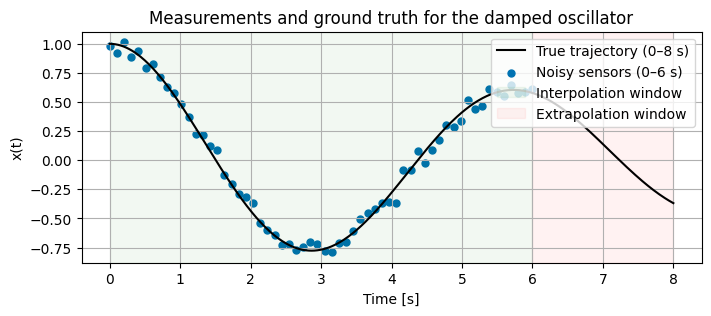
\includegraphics[width=0.85\linewidth]{09a-bnn-6-1.png}
\end{center}
\end{frame}

\begin{frame}
\frametitle{The challenge}
\begin{itemize}
    \item We observe noisy measurements $y_i = x(t_i) + \epsilon_i$ for $t \in [0, 6]$ s.
    \item We want predictions for $t \in [6, 8]$ s (extrapolation).
    \item \textbf{Key question}: How uncertain should we be about extrapolated predictions?
\end{itemize}
\vspace{0.3cm}
A standard NN would give a single curve with no uncertainty. \\
A Bayesian approach gives a \emph{distribution} over predictions.
\end{frame}

%========================================================================================
\section{Probability Distributions Primer}
%========================================================================================

\begin{frame}
\frametitle{Building blocks: probability distributions}
Bayesian models require specifying distributions. Three families cover most needs:
\begin{itemize}
    \item \textbf{Normal} $\mathcal{N}(\mu, \sigma^2)$: measurement noise, weight priors
    \item \textbf{Gamma} $\text{Gamma}(\alpha, \beta)$: positive scales, precisions
    \item \textbf{Uniform} $\text{Uniform}(a, b)$: weakly informative bounded priors
\end{itemize}
\end{frame}

\begin{frame}
\frametitle{The Normal distribution}
\[
p(x|\mu, \sigma^2) = \frac{1}{\sqrt{2\pi\sigma^2}} \exp\left(-\frac{(x-\mu)^2}{2\sigma^2}\right)
\]
\begin{center}
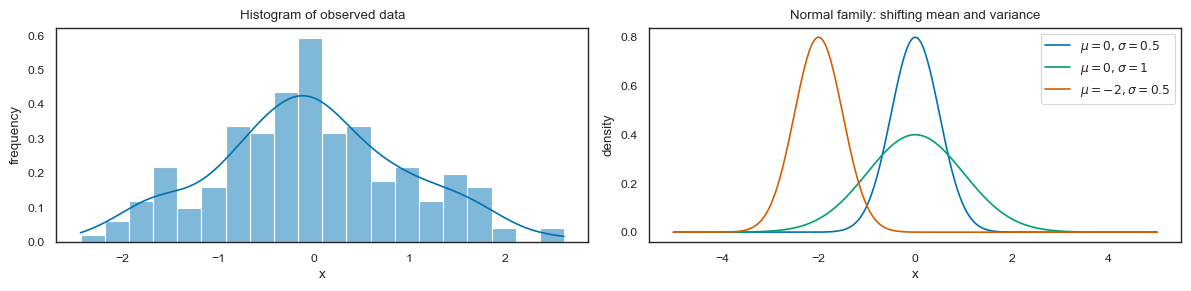
\includegraphics[width=0.9\linewidth]{09a-bnn-8-2.png}
\end{center}
\begin{itemize}
    \item $\mu$ shifts the center, $\sigma$ controls spread.
    \item Ubiquitous: Central Limit Theorem, maximum entropy for fixed variance.
\end{itemize}
\end{frame}

\begin{frame}
\frametitle{Gamma and Uniform distributions}
\begin{center}
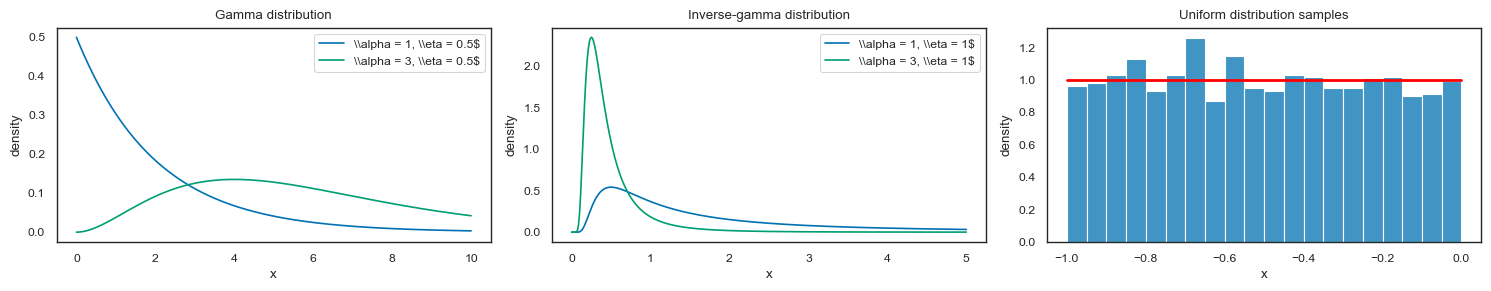
\includegraphics[width=0.95\linewidth]{09a-bnn-8-3.png}
\end{center}
\begin{itemize}
    \item \textbf{Gamma}: positive support, models precisions ($\tau = 1/\sigma^2$).
    \item \textbf{Inverse-Gamma}: conjugate prior for variance in Normal likelihood.
    \item \textbf{Uniform}: ``I only know the parameter lies in $[a,b]$.''
\end{itemize}
\end{frame}

%========================================================================================
\section{Bayes' Theorem}
%========================================================================================

\begin{frame}
\frametitle{Bayes' theorem: the update rule}
Given data $\mathcal{D}$ and parameters $\theta$:
\[
\underbrace{p(\theta|\mathcal{D})}_{\text{posterior}} = \frac{\overbrace{p(\mathcal{D}|\theta)}^{\text{likelihood}} \cdot \overbrace{p(\theta)}^{\text{prior}}}{\underbrace{p(\mathcal{D})}_{\text{evidence}}}
\]
\vspace{0.2cm}
\begin{itemize}
    \item \textbf{Prior} $p(\theta)$: what we believe before seeing data.
    \item \textbf{Likelihood} $p(\mathcal{D}|\theta)$: probability of data given parameters.
    \item \textbf{Posterior} $p(\theta|\mathcal{D})$: updated belief after seeing data.
    \item \textbf{Evidence} $p(\mathcal{D})$: normalizing constant (model comparison).
\end{itemize}
\end{frame}

\begin{frame}
\frametitle{Bayes on the oscillator: setup}
\textbf{Prior beliefs} (before seeing data):
\begin{itemize}
    \item Damping: $\zeta \sim \text{Uniform}(0, 0.25)$ --- light to moderate damping
    \item Frequency: $\omega_n \sim \text{Uniform}(0.6, 1.6)$ rad/s
\end{itemize}
\vspace{0.3cm}
\textbf{Likelihood} (how data relates to parameters):
\[
p(\mathcal{D}|\zeta, \omega_n) = \prod_{i=1}^{N} \mathcal{N}\bigl(y_i \,|\, x(t_i; \zeta, \omega_n), \sigma^2\bigr)
\]
where $x(t; \zeta, \omega_n)$ is the ODE solution.
\end{frame}

\begin{frame}
\frametitle{Bayes on the oscillator: posterior}
\[
p(\zeta, \omega_n | \mathcal{D}) \propto p(\mathcal{D}|\zeta, \omega_n) \cdot p(\zeta) \cdot p(\omega_n)
\]
\begin{center}
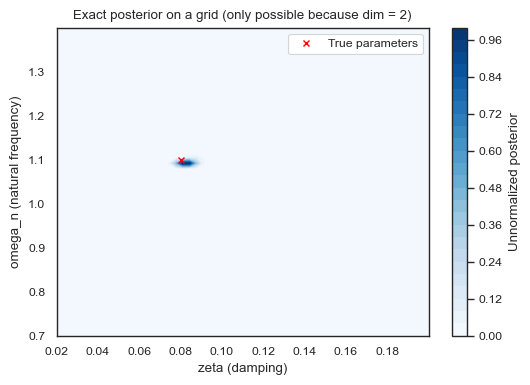
\includegraphics[width=0.5\linewidth]{09a-bnn-10-4.png}
\end{center}
\begin{itemize}
    \item Grid evaluation feasible because $\dim(\theta) = 2$.
    \item Posterior concentrates near true values $(\zeta=0.08, \omega_n=1.1)$.
    \item Uncertainty reflects noise level and data coverage.
\end{itemize}
\end{frame}

\begin{frame}
\frametitle{The curse of dimensionality}
Grid evaluation worked for 2 parameters. But:
\begin{itemize}
    \item Neural network with 1000 weights $\Rightarrow$ $10^{1000}$ grid points needed!
    \item Even MCMC struggles in high dimensions.
\end{itemize}
\vspace{0.3cm}
\textbf{Solution}: Variational inference --- approximate the posterior with a tractable distribution and optimize.
\vspace{0.3cm}

But first, let's understand exact Bayesian inference in a simpler setting...
\end{frame}

%========================================================================================
\section{Bayesian Linear Regression}
%========================================================================================

\begin{frame}
\frametitle{Why start with linear regression?}
Bayesian linear regression is the \textbf{only} case where:
\begin{enumerate}
    \item Posterior is available in closed form (no approximation needed).
    \item Predictive distribution is analytically tractable.
    \item We can visualize exactly what ``Bayesian'' means.
\end{enumerate}
\vspace{0.3cm}
The intuitions carry over to neural networks, where we must approximate.
\end{frame}

\begin{frame}
\frametitle{Model setup}
\textbf{Likelihood}: Linear model with Gaussian noise
\[
y = \mathbf{w}^T \boldsymbol{\phi}(\mathbf{x}) + \epsilon, \quad \epsilon \sim \mathcal{N}(0, \beta^{-1})
\]
where $\boldsymbol{\phi}(\mathbf{x}) = [1, \phi_1(\mathbf{x}), \ldots, \phi_{M-1}(\mathbf{x})]^T$ are basis functions.

\vspace{0.3cm}
\textbf{Prior}: Gaussian on weights
\[
p(\mathbf{w}) = \mathcal{N}(\mathbf{0}, \alpha^{-1}\mathbf{I})
\]
\begin{itemize}
    \item $\alpha$ = prior precision (large $\alpha$ $\Rightarrow$ weights close to zero).
    \item $\beta$ = noise precision (large $\beta$ $\Rightarrow$ low noise).
\end{itemize}
\end{frame}

\begin{frame}
\frametitle{Posterior derivation}
With $N$ observations $\{(\mathbf{x}_i, y_i)\}$, define design matrix $\boldsymbol{\Phi}$ with rows $\boldsymbol{\phi}(\mathbf{x}_i)^T$.

\vspace{0.2cm}
\textbf{Posterior} (Gaussian $\times$ Gaussian = Gaussian):
\[
p(\mathbf{w}|\mathcal{D}) = \mathcal{N}(\mathbf{m}_N, \mathbf{S}_N)
\]
where:
\[
\mathbf{S}_N^{-1} = \alpha\mathbf{I} + \beta\boldsymbol{\Phi}^T\boldsymbol{\Phi}, \qquad \mathbf{m}_N = \beta\mathbf{S}_N\boldsymbol{\Phi}^T\mathbf{t}
\]

\vspace{0.2cm}
\begin{itemize}
    \item $\mathbf{m}_N$: posterior mean (regularized least squares solution).
    \item $\mathbf{S}_N$: posterior covariance (uncertainty in weights).
\end{itemize}
\end{frame}

\begin{frame}
\frametitle{Predictive distribution}
For a new input $\mathbf{x}_*$, integrate over weight uncertainty:
\[
p(y_*|\mathbf{x}_*, \mathcal{D}) = \int p(y_*|\mathbf{x}_*, \mathbf{w}) \, p(\mathbf{w}|\mathcal{D}) \, d\mathbf{w}
\]
\vspace{0.2cm}
Result (Gaussian):
\[
p(y_*|\mathbf{x}_*, \mathcal{D}) = \mathcal{N}\bigl(\mathbf{m}_N^T\boldsymbol{\phi}_*, \; \sigma_*^2\bigr)
\]
where:
\[
\sigma_*^2 = \underbrace{\beta^{-1}}_{\text{noise}} + \underbrace{\boldsymbol{\phi}_*^T \mathbf{S}_N \boldsymbol{\phi}_*}_{\text{weight uncertainty}}
\]
\end{frame}

\begin{frame}
\frametitle{Two sources of uncertainty}
\[
\sigma_*^2 = \underbrace{\beta^{-1}}_{\text{aleatoric}} + \underbrace{\boldsymbol{\phi}_*^T \mathbf{S}_N \boldsymbol{\phi}_*}_{\text{epistemic}}
\]
\vspace{0.2cm}
\begin{itemize}
    \item \textbf{Aleatoric uncertainty} ($\beta^{-1}$): irreducible noise in the data. Cannot be reduced by collecting more data.
    \item \textbf{Epistemic uncertainty} ($\boldsymbol{\phi}_*^T \mathbf{S}_N \boldsymbol{\phi}_*$): uncertainty about model parameters. \emph{Shrinks} as we collect more data.
\end{itemize}
\vspace{0.3cm}
This decomposition is central to Bayesian approaches!
\end{frame}

\begin{frame}
\frametitle{Posterior evolution with data}
\begin{center}
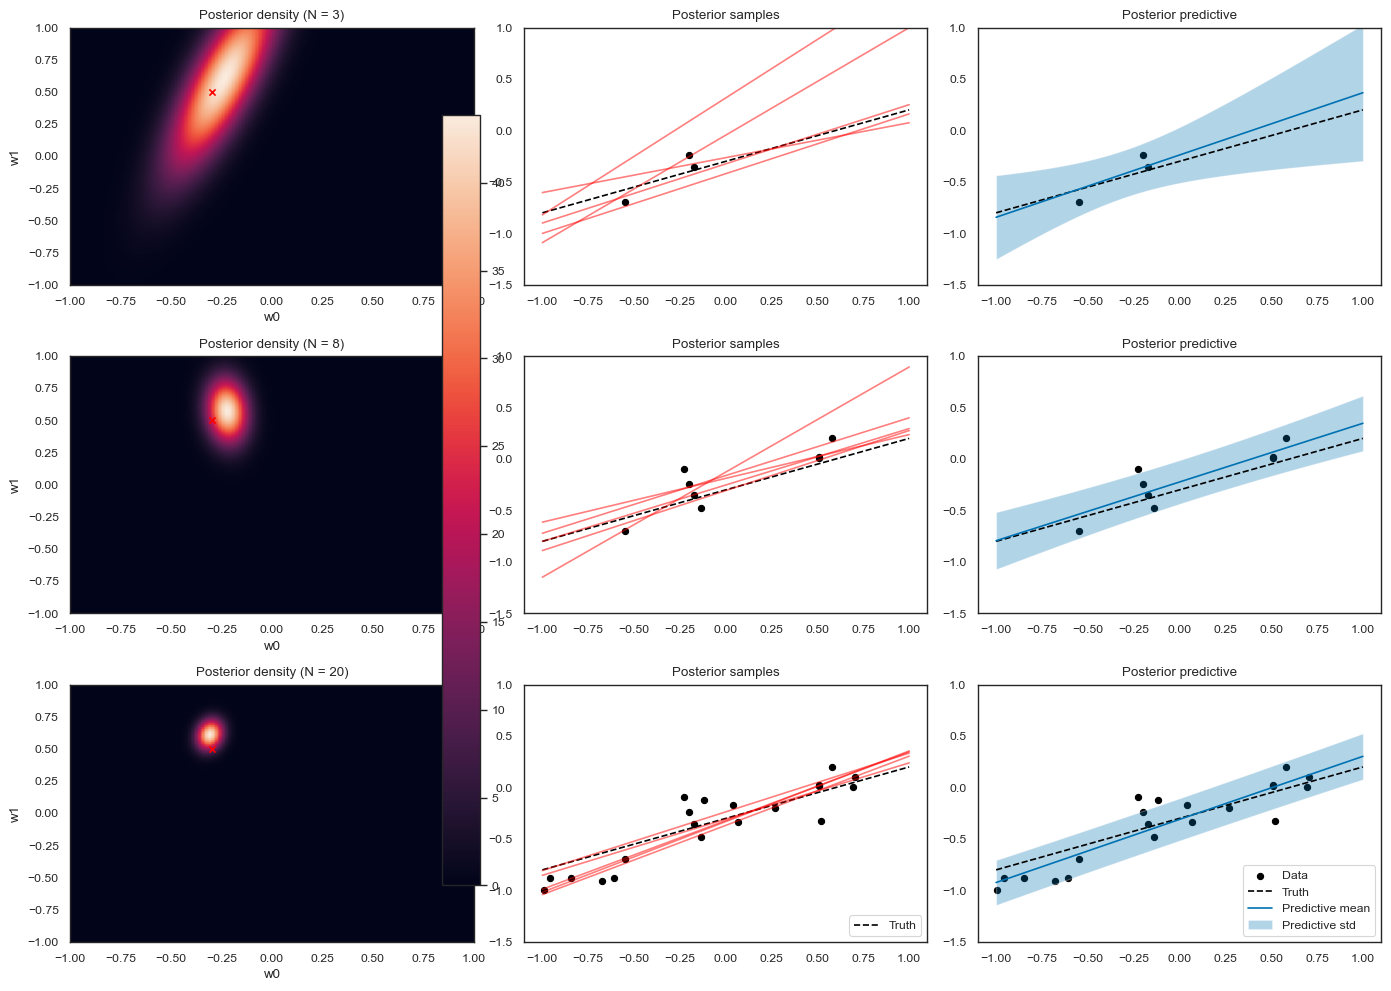
\includegraphics[width=0.75\linewidth]{09a-bnn-13-5.png}
\end{center}
\vspace{-0.2cm}
\begin{itemize}
    \item \textbf{Left}: Posterior density over weights sharpens with more data.
    \item \textbf{Middle}: Posterior samples of functions become more consistent.
    \item \textbf{Right}: Predictive bands shrink where data exist.
\end{itemize}
\end{frame}

\begin{frame}
\frametitle{Nonlinear targets via basis functions}
Replace identity basis with Gaussian basis: $\phi_j(x) = \exp\bigl(-\frac{(x - \mu_j)^2}{2\sigma^2}\bigr)$
\begin{center}
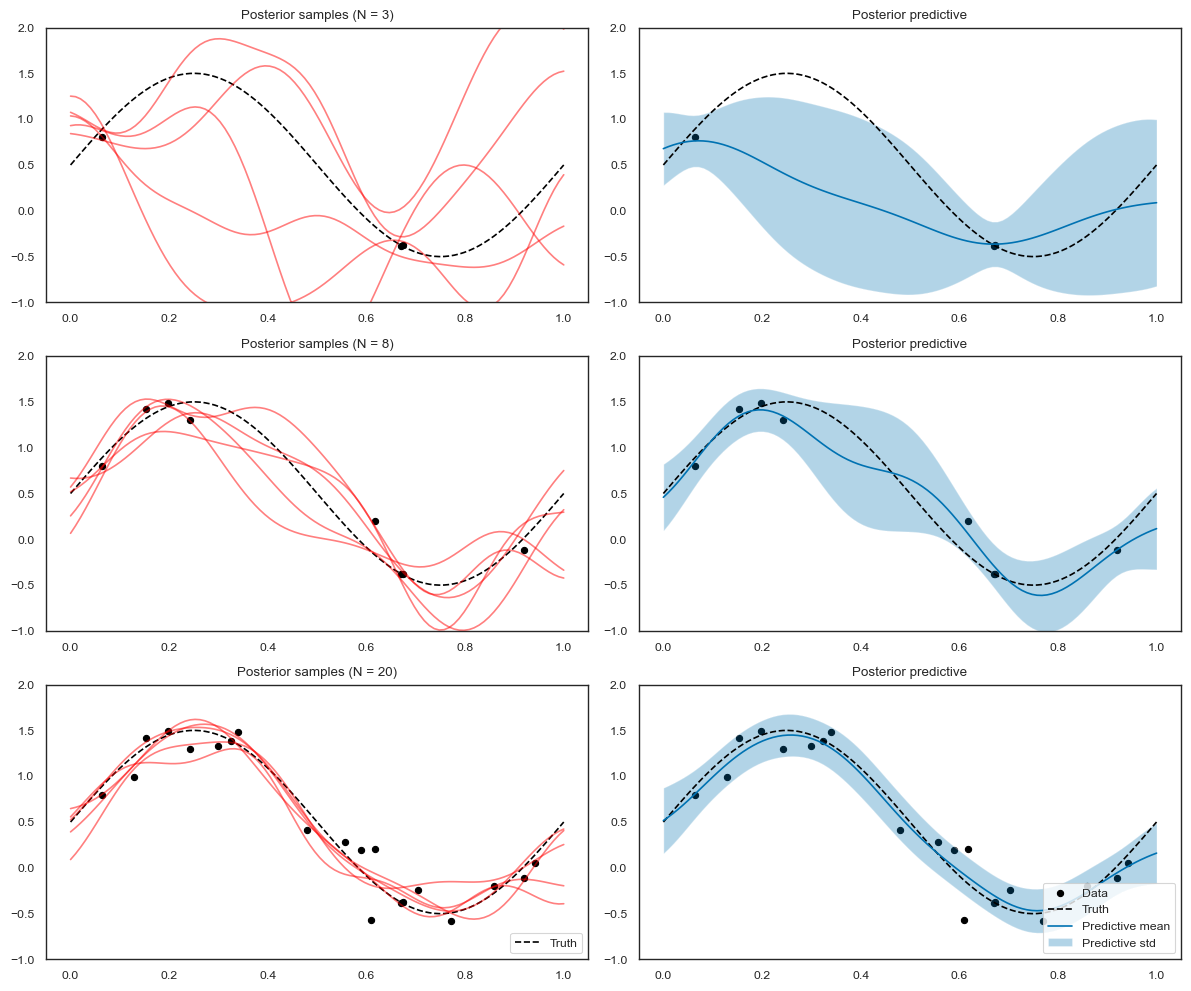
\includegraphics[width=0.58\linewidth]{09a-bnn-14-6.png}
\end{center}
Linear model in $\boldsymbol{\phi}$ space fits nonlinear targets in $x$ space.
\end{frame}

\begin{frame}
\frametitle{Key observation: uncertainty away from data}
\begin{center}
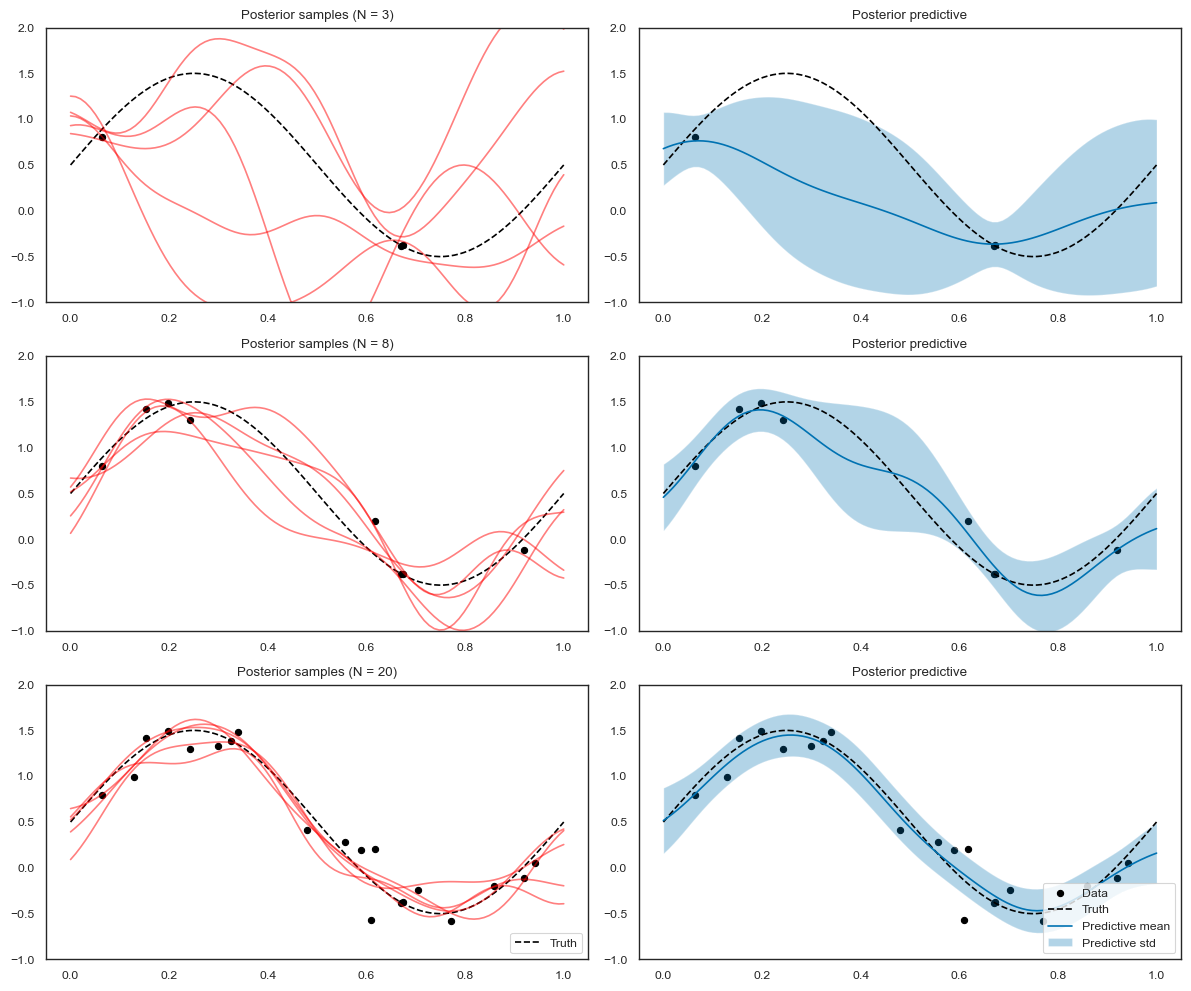
\includegraphics[width=0.55\linewidth]{09a-bnn-14-6.png}
\end{center}
\begin{itemize}
    \item Predictive bands are \textbf{tight} near observations.
    \item Bands \textbf{widen} away from data (epistemic uncertainty grows).
    \item This is exactly what we want for extrapolation warnings!
\end{itemize}
\end{frame}

%========================================================================================
\section{Model Selection via Evidence}
%========================================================================================

\begin{frame}
\frametitle{The model selection problem}
How do we choose:
\begin{itemize}
    \item Number of basis functions?
    \item Polynomial degree?
    \item Network architecture?
\end{itemize}
\vspace{0.3cm}
Cross-validation is one approach. Bayesian model selection uses the \textbf{evidence} (marginal likelihood):
\[
p(\mathcal{D}|\mathcal{M}) = \int p(\mathcal{D}|\theta, \mathcal{M}) \, p(\theta|\mathcal{M}) \, d\theta
\]
\end{frame}

\begin{frame}
\frametitle{Evidence as automatic Occam's razor}
\[
\ln p(\mathbf{t}|\alpha,\beta) = \underbrace{\frac{M}{2}\ln\alpha + \frac{N}{2}\ln\beta - E(\mathbf{m}_N)}_{\text{data fit}} - \underbrace{\frac{1}{2}\ln|\mathbf{S}_N^{-1}|}_{\text{complexity}} - \frac{N}{2}\ln(2\pi)
\]
\vspace{0.2cm}
\begin{itemize}
    \item Complex models can fit data well but have low prior probability for any specific fit.
    \item Simple models have high prior probability but may not fit data.
    \item Evidence balances automatically --- no tuning needed.
\end{itemize}
\end{frame}

\begin{frame}
\frametitle{Evidence in action: polynomial regression}
\begin{columns}[T]
\column{0.6\textwidth}
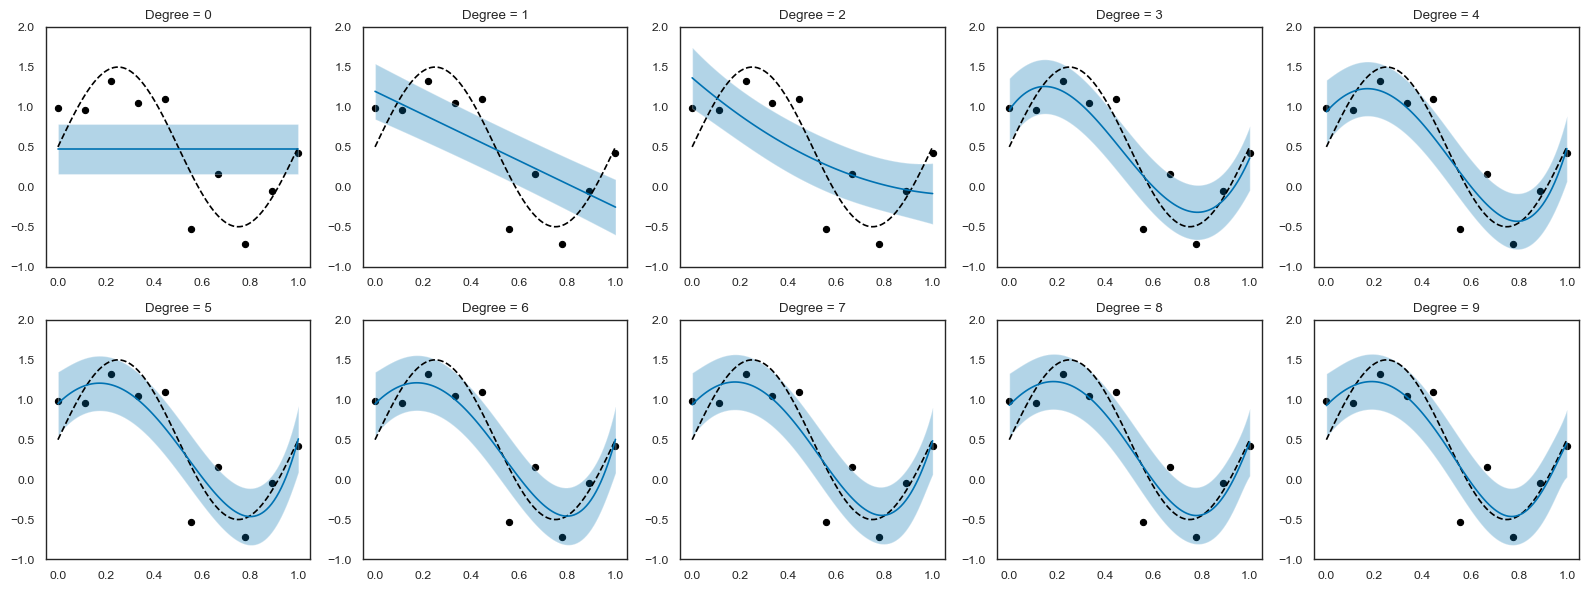
\includegraphics[width=\linewidth]{09a-bnn-16-7.png}
\column{0.4\textwidth}
\vspace{0.3cm}
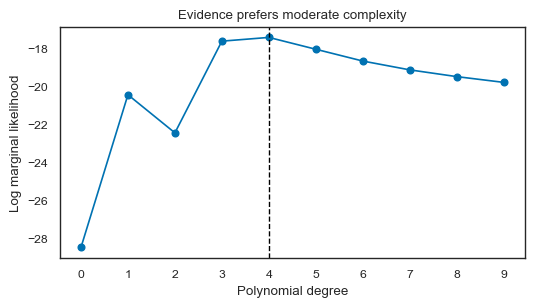
\includegraphics[width=\linewidth]{09a-bnn-16-8.png}
\vspace{0.2cm}
\begin{itemize}
\item Peak at degree 3.
\item Lower degrees: underfit.
\item Higher degrees: overfit.
\end{itemize}
\end{columns}
\end{frame}

\begin{frame}
\frametitle{Empirical Bayes}
We can also optimize hyperparameters $\alpha, \beta$ by maximizing evidence:
\[
\alpha^*, \beta^* = \arg\max_{\alpha, \beta} \ln p(\mathcal{D}|\alpha, \beta)
\]
\vspace{0.2cm}
\begin{itemize}
    \item Called ``Empirical Bayes'' or ``Type II Maximum Likelihood.''
    \item Automatic regularization strength selection.
    \item No cross-validation needed.
\end{itemize}
\end{frame}

%========================================================================================
\section{Variational Inference}
%========================================================================================

\begin{frame}
\frametitle{The scalability problem}
Bayesian linear regression works because:
\begin{itemize}
    \item Gaussian prior $\times$ Gaussian likelihood $=$ Gaussian posterior.
\end{itemize}
\vspace{0.3cm}
For neural networks:
\begin{itemize}
    \item Posterior $p(\mathbf{w}|\mathcal{D})$ is \textbf{intractable} (no closed form).
    \item MCMC is too slow for millions of parameters.
    \item We need a fast approximation.
\end{itemize}
\vspace{0.3cm}
\textbf{Variational inference}: Approximate $p(\mathbf{w}|\mathcal{D})$ with a tractable $q_\phi(\mathbf{w})$.
\end{frame}

\begin{frame}
\frametitle{The variational objective}
Find $q_\phi(\mathbf{w})$ that is ``close'' to $p(\mathbf{w}|\mathcal{D})$ by minimizing KL divergence:
\[
\text{KL}(q_\phi \| p(\cdot|\mathcal{D})) = \int q_\phi(\mathbf{w}) \ln \frac{q_\phi(\mathbf{w})}{p(\mathbf{w}|\mathcal{D})} d\mathbf{w}
\]
\vspace{0.2cm}
Problem: This requires knowing $p(\mathbf{w}|\mathcal{D})$, which is intractable!
\vspace{0.3cm}

Solution: Rearrange to get the \textbf{Evidence Lower Bound (ELBO)}.
\end{frame}

\begin{frame}
\frametitle{Deriving the ELBO}
Start with log evidence:
\[
\ln p(\mathcal{D}) = \ln \int p(\mathcal{D}, \mathbf{w}) \, d\mathbf{w}
\]
Multiply and divide by $q_\phi(\mathbf{w})$, apply Jensen's inequality:
\[
\ln p(\mathcal{D}) \geq \underbrace{\mathbb{E}_{q_\phi}\bigl[\ln p(\mathcal{D}|\mathbf{w})\bigr]}_{\text{expected log-likelihood}} - \underbrace{\text{KL}(q_\phi \| p(\mathbf{w}))}_{\text{complexity penalty}}
\]
This is the \textbf{ELBO} $\mathcal{L}(\phi)$. Maximizing ELBO $\Leftrightarrow$ minimizing KL to posterior.
\end{frame}

\begin{frame}
\frametitle{ELBO intuition}
\[
\mathcal{L}(\phi) = \underbrace{\mathbb{E}_{q_\phi}[\ln p(\mathcal{D}|\mathbf{w})]}_{\text{data fit}} - \underbrace{\text{KL}(q_\phi \| p(\mathbf{w}))}_{\text{stay close to prior}}
\]
\vspace{0.3cm}
\begin{itemize}
    \item \textbf{First term}: Encourages $q_\phi$ to put mass on weights that explain data.
    \item \textbf{Second term}: Penalizes $q_\phi$ for deviating from prior (regularization).
\end{itemize}
\vspace{0.3cm}
Same trade-off as MAP estimation, but for entire distributions!
\end{frame}

\begin{frame}
\frametitle{The reparameterization trick}
To optimize ELBO with gradient descent, we need $\nabla_\phi \mathbb{E}_{q_\phi}[f(\mathbf{w})]$.
\vspace{0.2cm}

\textbf{Problem}: Expectation depends on $\phi$ through the distribution.
\vspace{0.2cm}

\textbf{Solution}: Reparameterize the sampling:
\[
\mathbf{w} = \boldsymbol{\mu} + \boldsymbol{\sigma} \odot \boldsymbol{\epsilon}, \quad \boldsymbol{\epsilon} \sim \mathcal{N}(\mathbf{0}, \mathbf{I})
\]
Now $\mathbf{w}$ is a deterministic function of $\phi = \{\boldsymbol{\mu}, \boldsymbol{\sigma}\}$ and random $\boldsymbol{\epsilon}$:
\[
\nabla_\phi \mathbb{E}_{q_\phi}[f(\mathbf{w})] = \mathbb{E}_{\boldsymbol{\epsilon}}[\nabla_\phi f(\boldsymbol{\mu} + \boldsymbol{\sigma} \odot \boldsymbol{\epsilon})]
\]
\end{frame}

\begin{frame}
\frametitle{VI example: approximating a bimodal posterior}
\begin{center}
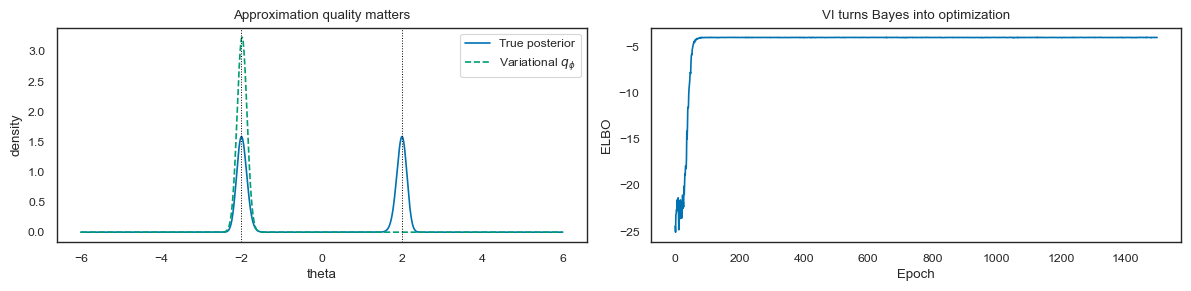
\includegraphics[width=0.85\linewidth]{09a-bnn-18-9.png}
\end{center}
\begin{itemize}
    \item True posterior is bimodal (two plausible values of $\theta$).
    \item Single Gaussian $q_\phi$ can only capture one mode.
    \item This is the \textbf{mean-field approximation} limitation.
\end{itemize}
\end{frame}

\begin{frame}
\frametitle{Mean-field approximation}
For computational tractability, we assume:
\[
q_\phi(\mathbf{w}) = \prod_{i} q_{\phi_i}(w_i) = \prod_i \mathcal{N}(w_i | \mu_i, \sigma_i^2)
\]
\vspace{0.2cm}
\begin{itemize}
    \item Each weight has independent Gaussian posterior.
    \item Ignores correlations between weights.
    \item Trades accuracy for scalability.
\end{itemize}
\vspace{0.3cm}
Despite limitations, works surprisingly well in practice!
\end{frame}

%========================================================================================
\section{Bayesian Neural Networks}
%========================================================================================

\begin{frame}
\frametitle{From VI to BNNs}
Apply variational inference to neural network weights:
\begin{enumerate}
    \item Replace each weight $w_{ij}$ with distribution $q(w_{ij}) = \mathcal{N}(\mu_{ij}, \sigma_{ij}^2)$.
    \item Define prior $p(\mathbf{w}) = \mathcal{N}(\mathbf{0}, \sigma_p^2 \mathbf{I})$.
    \item Optimize ELBO via stochastic gradient descent.
\end{enumerate}
\vspace{0.3cm}
This is \textbf{Bayes by Backprop} (Blundell et al., 2015).
\end{frame}

\begin{frame}
\frametitle{BayesianLinear layer}
Standard linear layer: $\mathbf{y} = \mathbf{W}\mathbf{x} + \mathbf{b}$ with fixed $\mathbf{W}, \mathbf{b}$.
\vspace{0.3cm}

Bayesian linear layer:
\begin{enumerate}
    \item Store $\mu_W, \rho_W, \mu_b, \rho_b$ (variational parameters).
    \item Compute $\sigma = \text{softplus}(\rho) = \ln(1 + e^\rho)$ (ensures $\sigma > 0$).
    \item Sample: $W = \mu_W + \sigma_W \odot \epsilon_W$, \; $\epsilon_W \sim \mathcal{N}(0, 1)$.
    \item Forward pass: $\mathbf{y} = \mathbf{W}\mathbf{x} + \mathbf{b}$.
    \item Compute KL term for loss.
\end{enumerate}
\end{frame}

\begin{frame}
\frametitle{Bayes by Backprop loss}
\vspace{-0.2cm}
\[
\mathcal{L} = \underbrace{\text{KL}(q_\phi(\mathbf{w}) \| p(\mathbf{w}))}_{\text{complexity cost}} - \underbrace{\mathbb{E}_{q_\phi}[\ln p(\mathcal{D}|\mathbf{w})]}_{\text{likelihood cost}}
\]
Monte Carlo estimate with $S$ weight samples:
\[
\mathcal{L} \approx \frac{1}{S}\sum_{s=1}^{S}\Bigl[\ln q_\phi(\mathbf{w}^{(s)}) - \ln p(\mathbf{w}^{(s)}) - \ln p(\mathcal{D}|\mathbf{w}^{(s)})\Bigr]
\]
\vspace{0.2cm}
\begin{itemize}
    \item Sample weights once (or few times) per minibatch.
    \item Backprop through sampled network as usual.
    \item Twice the parameters (mean + variance for each weight).
\end{itemize}
\end{frame}

\begin{frame}
\frametitle{Training the BNN surrogate}
\begin{center}
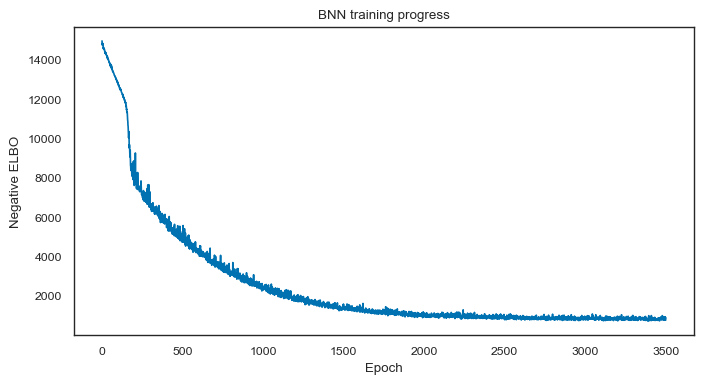
\includegraphics[width=0.6\linewidth]{09a-bnn-22-10.png}
\end{center}
\begin{itemize}
    \item Architecture: 1 $\to$ 64 $\to$ 64 $\to$ 1 with tanh activations.
    \item Prior: $\mathcal{N}(0, 1)$ on all weights.
    \item Training: 3500 epochs, Adam optimizer, 6 MC samples per step.
\end{itemize}
\end{frame}

\begin{frame}
\frametitle{Predictive distribution}
At test time, approximate predictive distribution via Monte Carlo:
\[
p(y_*|x_*, \mathcal{D}) \approx \frac{1}{S}\sum_{s=1}^{S} p(y_*|x_*, \mathbf{w}^{(s)}), \quad \mathbf{w}^{(s)} \sim q_\phi(\mathbf{w})
\]
\vspace{0.2cm}
In practice:
\begin{enumerate}
    \item Sample $S$ weight configurations from $q_\phi$.
    \item Run forward pass for each to get $S$ predictions.
    \item Compute mean and variance of predictions.
\end{enumerate}
\end{frame}

%========================================================================================
\section{Results: Interpolation vs Extrapolation}
%========================================================================================

\begin{frame}
\frametitle{BNN predictions with uncertainty}
\begin{center}
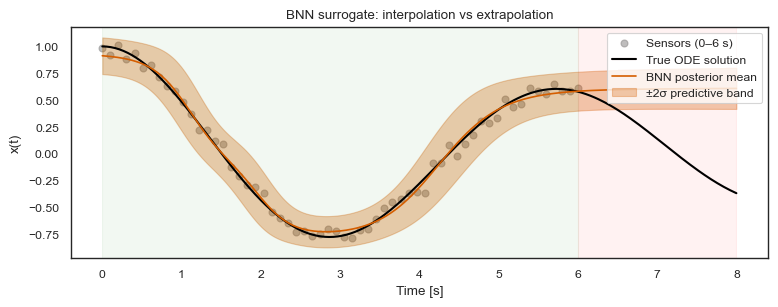
\includegraphics[width=0.9\linewidth]{09a-bnn-23-11.png}
\end{center}
\begin{itemize}
    \item \textbf{Green region} (0--6 s): Training data. Tight predictive bands.
    \item \textbf{Red region} (6--8 s): Extrapolation. Bands widen significantly.
\end{itemize}
\end{frame}

\begin{frame}
\frametitle{Why uncertainty grows in extrapolation}
\begin{itemize}
    \item In training region: Many weight configurations fit the data $\Rightarrow$ predictions agree.
    \item In extrapolation: Weight configurations that agreed on training data \textbf{diverge} outside it.
\end{itemize}
\vspace{0.3cm}
This is exactly what we want! The model \textbf{knows what it doesn't know}.
\end{frame}

\begin{frame}
\frametitle{Posterior samples tell the story}
\begin{center}
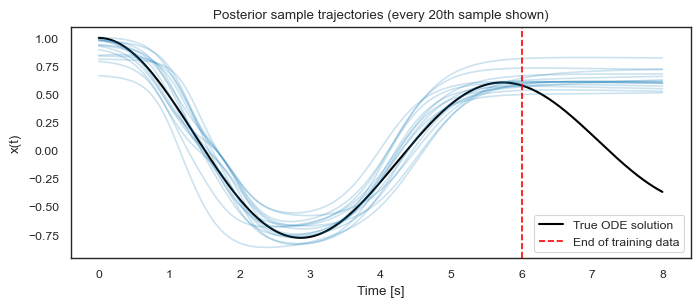
\includegraphics[width=0.95\linewidth]{09a-bnn-24-12.png}
\end{center}
\begin{itemize}
    \item Each curve: one forward pass with $\mathbf{w}^{(s)} \sim q_\phi(\mathbf{w})$.
    \item Curves cluster in training region, fan out when extrapolating.
    \item \textbf{Epistemic uncertainty} visualized directly.
\end{itemize}
\end{frame}

\begin{frame}
\frametitle{Epistemic vs Aleatoric uncertainty revisited}
\begin{itemize}
    \item \textbf{Aleatoric} (data noise): Present everywhere, irreducible.
    \item \textbf{Epistemic} (model uncertainty):
    \begin{itemize}
        \item Small where data exist (model is confident).
        \item Large in extrapolation (model is uncertain).
        \item Can be reduced with more data in those regions.
    \end{itemize}
\end{itemize}
\vspace{0.3cm}
BNNs naturally capture both through the predictive distribution.
\end{frame}

%========================================================================================
\section{Practical Considerations}
%========================================================================================

\begin{frame}
\frametitle{BNN limitations}
\begin{itemize}
    \item \textbf{Computational cost}: 2$\times$ parameters, multiple forward passes.
    \item \textbf{Mean-field approximation}: Ignores weight correlations.
    \item \textbf{Prior specification}: Results sensitive to prior choice.
    \item \textbf{Underestimated uncertainty}: VI tends to underestimate variance.
\end{itemize}
\end{frame}

\begin{frame}
\frametitle{Faster alternatives}
\textbf{MC Dropout} (Gal \& Ghahramani, 2016):
\begin{itemize}
    \item Keep dropout on at test time.
    \item Multiple forward passes $\approx$ posterior samples.
    \item No architecture changes needed!
\end{itemize}
\vspace{0.3cm}
\textbf{Deep Ensembles} (Lakshminarayanan et al., 2017):
\begin{itemize}
    \item Train $M$ networks with different initializations.
    \item Ensemble variance $\approx$ epistemic uncertainty.
    \item Often outperforms BNNs in practice.
\end{itemize}
\end{frame}

\begin{frame}
\frametitle{When to use BNNs}
\textbf{Good fit for BNNs}:
\begin{itemize}
    \item Small to medium datasets where uncertainty matters.
    \item Safety-critical applications (medical, autonomous systems).
    \item Active learning (query where uncertainty is high).
    \item Scientific ML: need calibrated extrapolation warnings.
\end{itemize}
\vspace{0.3cm}
\textbf{Consider alternatives}:
\begin{itemize}
    \item Large-scale vision/NLP (use ensembles or MC dropout).
    \item When computational budget is very limited.
\end{itemize}
\end{frame}

%========================================================================================
\section{Summary}
%========================================================================================

\begin{frame}
\frametitle{Key takeaways}
\begin{enumerate}
    \item \textbf{Bayes' theorem} provides a principled framework for updating beliefs with data.
    \item \textbf{Bayesian linear regression} gives exact posteriors --- study it to build intuition.
    \item \textbf{Evidence} automatically balances model fit vs complexity.
    \item \textbf{Variational inference} turns Bayesian inference into optimization.
    \item \textbf{BNNs} provide calibrated uncertainty, especially for extrapolation.
\end{enumerate}
\end{frame}

\begin{frame}
\frametitle{The big picture}
\begin{center}
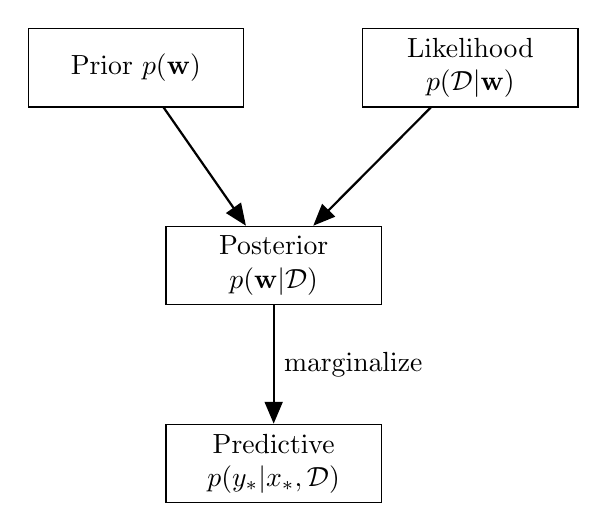
\begin{tikzpicture}[node distance=1.5cm, auto,
    box/.style={rectangle, draw, text width=2.5cm, align=center, minimum height=1cm}]
    \node[box] (prior) {Prior $p(\mathbf{w})$};
    \node[box, right=of prior] (likelihood) {Likelihood $p(\mathcal{D}|\mathbf{w})$};
    \node[box, below=of prior, xshift=1.75cm] (posterior) {Posterior $p(\mathbf{w}|\mathcal{D})$};
    \node[box, below=of posterior] (predictive) {Predictive $p(y_*|x_*, \mathcal{D})$};

    \draw[->, thick] (prior) -- (posterior);
    \draw[->, thick] (likelihood) -- (posterior);
    \draw[->, thick] (posterior) -- (predictive) node[midway, right] {marginalize};
\end{tikzpicture}
\end{center}
\vspace{0.3cm}
BNNs approximate this pipeline with variational inference, giving us uncertainty-aware predictions for scientific machine learning.
\end{frame}

\begin{frame}
\frametitle{Further reading}
\begin{itemize}
    \item \textbf{Bishop, PRML Ch. 3}: Bayesian linear regression derivations.
    \item \textbf{Blundell et al. (2015)}: ``Weight Uncertainty in Neural Networks'' --- Bayes by Backprop.
    \item \textbf{Gal \& Ghahramani (2016)}: ``Dropout as a Bayesian Approximation.''
    \item \textbf{Lakshminarayanan et al. (2017)}: ``Simple and Scalable Predictive Uncertainty Estimation using Deep Ensembles.''
\end{itemize}
\vspace{0.3cm}
\textbf{Code}: See accompanying notebook \texttt{09a-bnn.ipynb} for full implementation.
\end{frame}

\end{document}
